\chapter{Dataset Description and System Architecture}
\section{Dataset Overview}
The project uses a preprocessed Human Activity Recognition dataset containing feature vectors and activity labels. The files supplied for the project include the training and testing feature matrices (\texttt{X\_train.txt}, \texttt{X\_test.txt}), the corresponding target labels (\texttt{y\_train.txt}, \texttt{y\_test.txt}), a feature-name file and an activity-label mapping file.

\begin{table}[H]
\centering
\caption{Dataset dimensions used in the project}
\begin{tabular}{lr}
\toprule
\textbf{Dataset component} & \textbf{Number of records / features}\\
\midrule
Training observations & 7,352\\
Testing observations & 2,947\\
Total observations & 10,299\\
Input features per observation & 561\\
Activity classes & 6\\
\bottomrule
\end{tabular}
\end{table}

\emph{The training matrix therefore has dimensions $7352 \times 561$, while the test matrix has dimensions $2947 \times 561$.} The target vectors contain one integer activity identifier for each corresponding observation.

\section{Activity Labels}
\begin{table}[H]
\centering
\caption{Activity identifiers and their meanings}
\begin{tabular}{cl}
\toprule
\textbf{Identifier} & \textbf{Activity}\\
\midrule
1 & WALKING\\
2 & WALKING\_UPSTAIRS\\
3 & WALKING\_DOWNSTAIRS\\
4 & SITTING\\
5 & STANDING\\
6 & LAYING\\
\bottomrule
\end{tabular}
\end{table}

\section{Feature Description}
The supplied feature information describes variables derived from three-axis accelerometer and gyroscope signals sampled at 50 Hz. The documented signal processing includes median filtering and a third-order low-pass Butterworth filter with a 20 Hz corner frequency. Acceleration is separated into body acceleration and gravity acceleration using a low-pass Butterworth filter with a 0.3 Hz corner frequency. Jerk signals are derived from body acceleration and angular velocity. Signal magnitudes are calculated using the Euclidean norm, and Fast Fourier Transform (FFT) features are generated for selected signals.

The feature set includes statistical and signal descriptors such as mean, standard deviation, median absolute deviation, maximum, minimum, signal magnitude area, energy, interquartile range, entropy, autoregression coefficients, correlation, frequency-related descriptors and angles. The complete list of 561 feature names is provided in the supplied \texttt{features.txt} file.

\textbf{Implementation clarification:} These signal-processing operations are described in the supplied feature documentation as the origin of the prepared features. \emph{The submitted notebook loads the already-computed 561-dimensional feature matrices. It does not independently apply the raw-signal filtering or FFT steps to sensor recordings.}

\section{Data Quality Checks}
The notebook checks the training and test feature matrices for missing values, duplicate rows and finite numerical values. The recorded results are:
\begin{itemize}
\item Missing values in training data: 0.
\item Missing values in testing data: 0.
\item Duplicate rows in training data: 0.
\item Duplicate rows in testing data: 0.
\item \emph{All values in both matrices are finite.}
\end{itemize}

\section{Activity Distribution}
Figure~\ref{fig:activitydist} compares the number of samples in each class across the training and testing partitions. The training counts are 1,226 (walking), 1,073 (walking upstairs), 986 (walking downstairs), 1,286 (sitting), 1,374 (standing) and 1,407 (laying). The corresponding test counts are 496, 471, 420, 491, 532 and 537.

\begin{figure}[H]
\centering
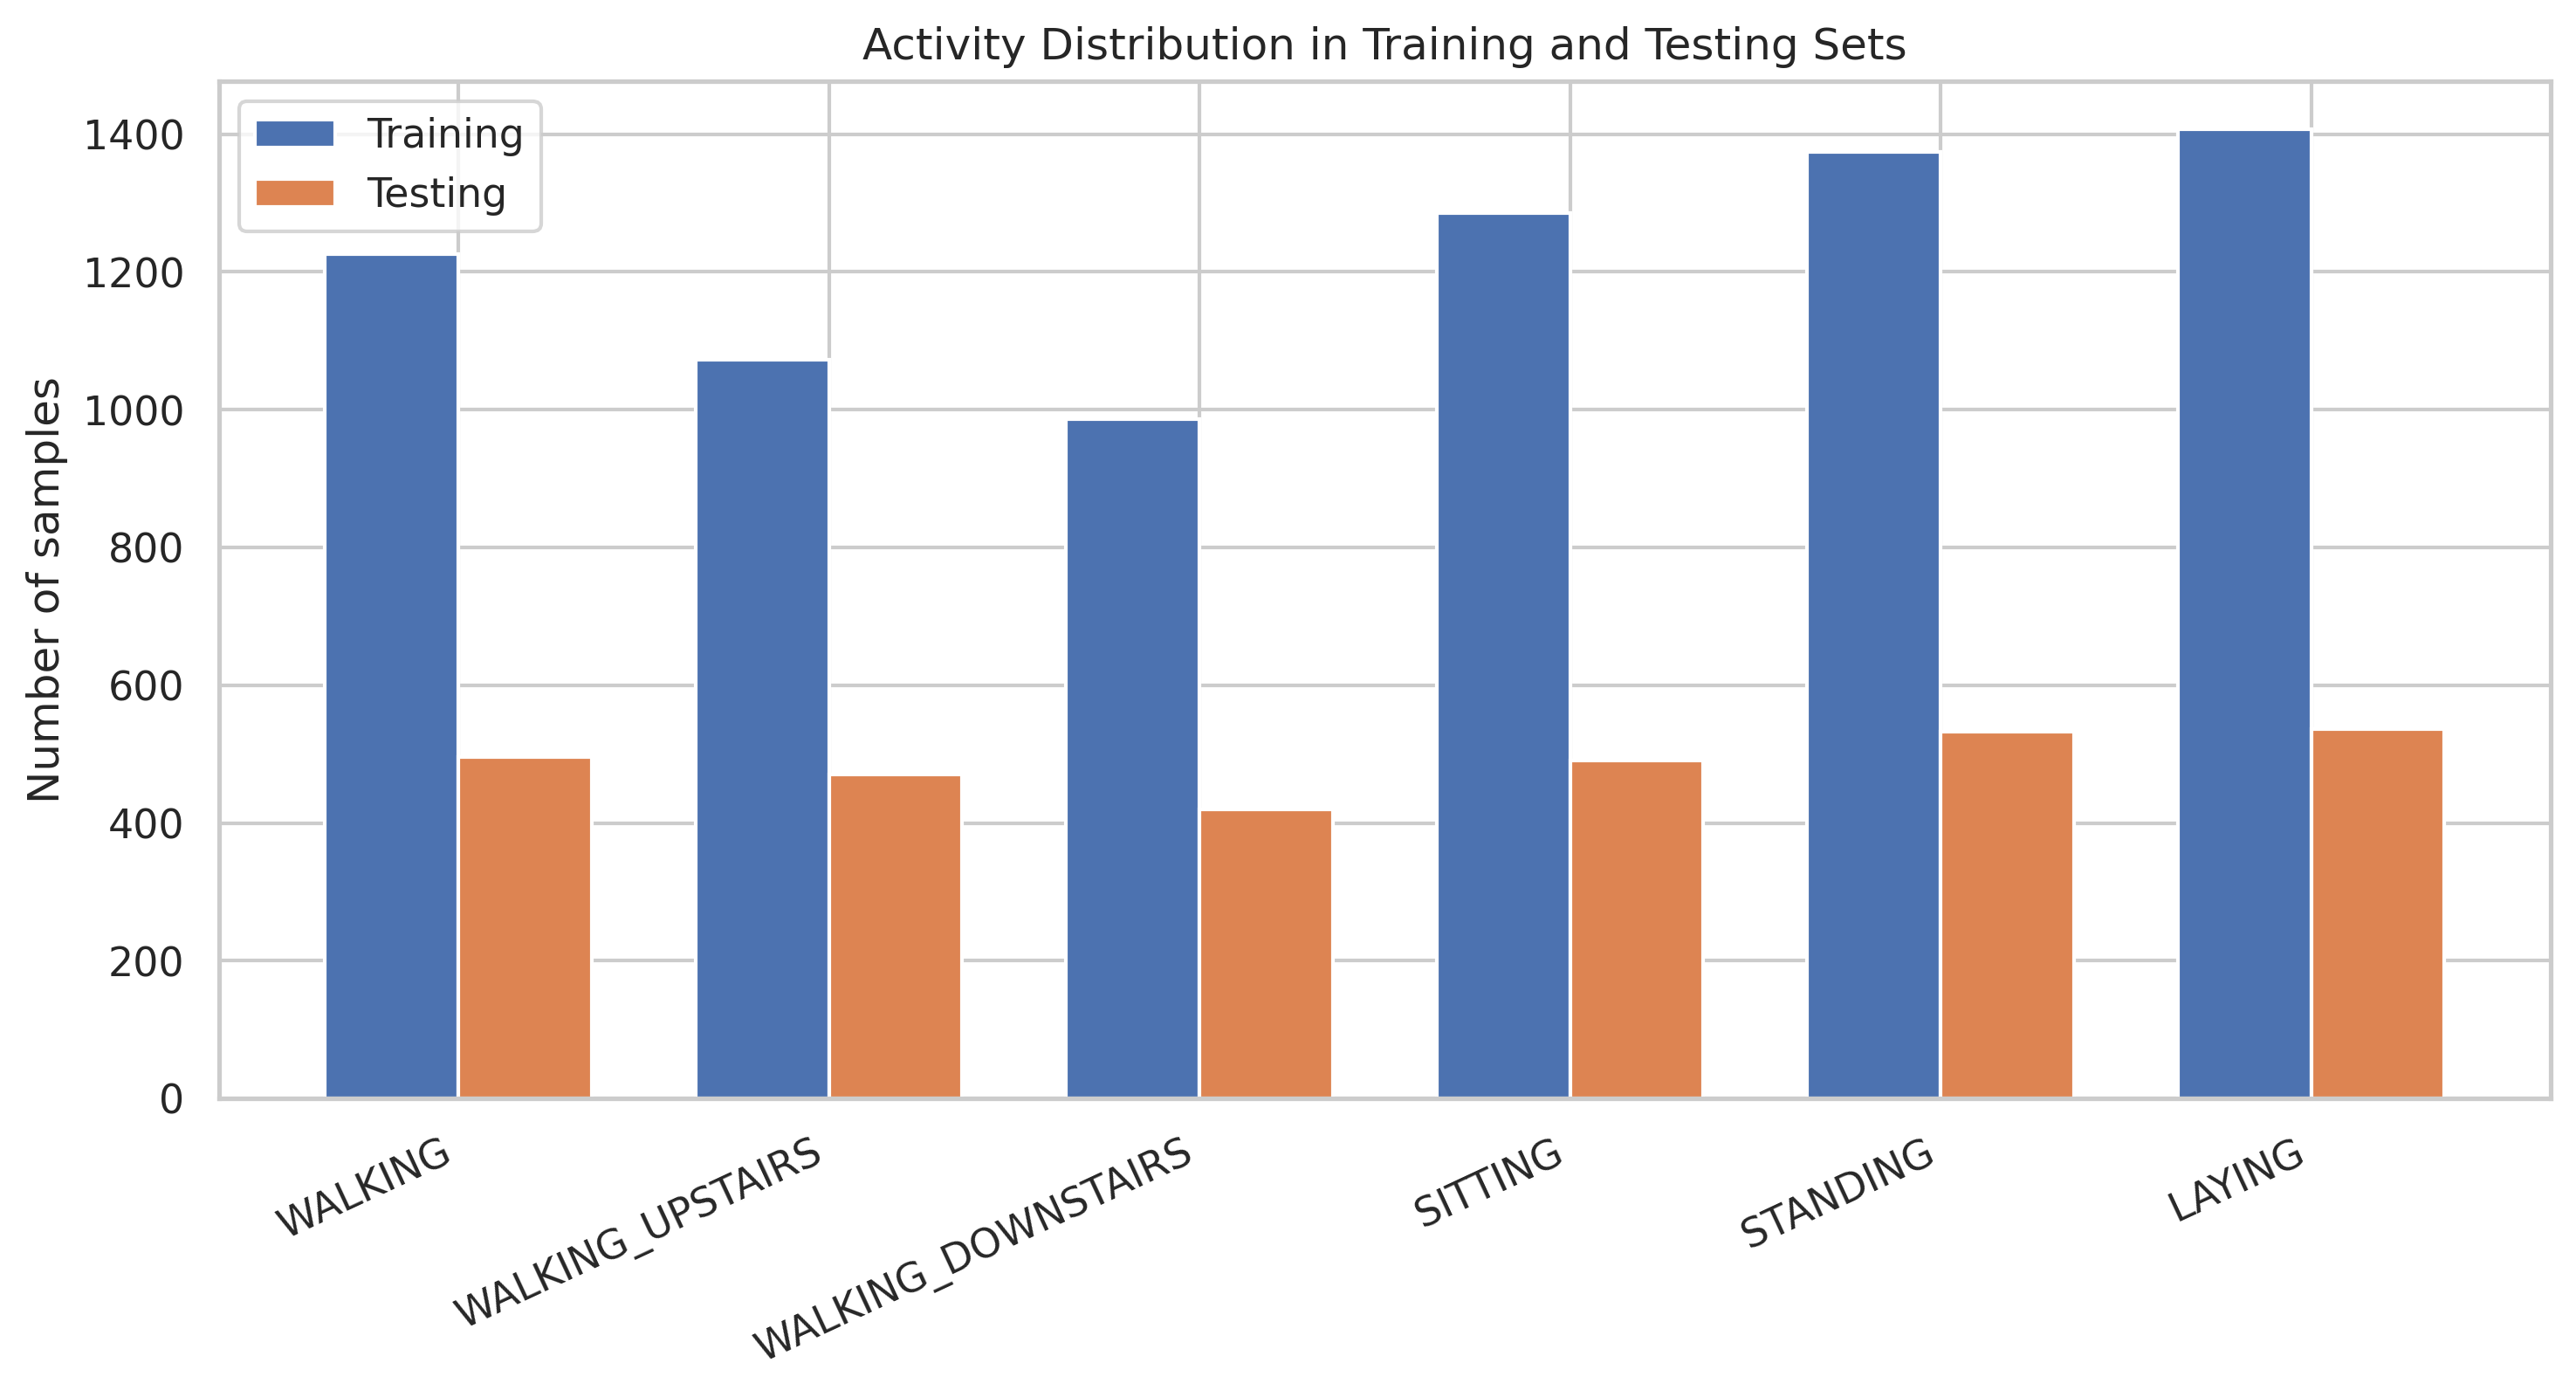
\includegraphics[width=0.92\textwidth]{activity_distribution.png}
\caption{Activity distribution in the training and testing datasets.}
\label{fig:activitydist}
\end{figure}

\section{Proposed System Architecture}
The project workflow starts with the prepared HAR dataset and feature-label mapping. After loading and data-quality checks, the feature matrices are passed to three supervised classifiers. Predictions are evaluated using quantitative metrics and visual analysis. The trained models and metadata are exported as artifacts for the web application.

\begin{figure}[H]
\centering
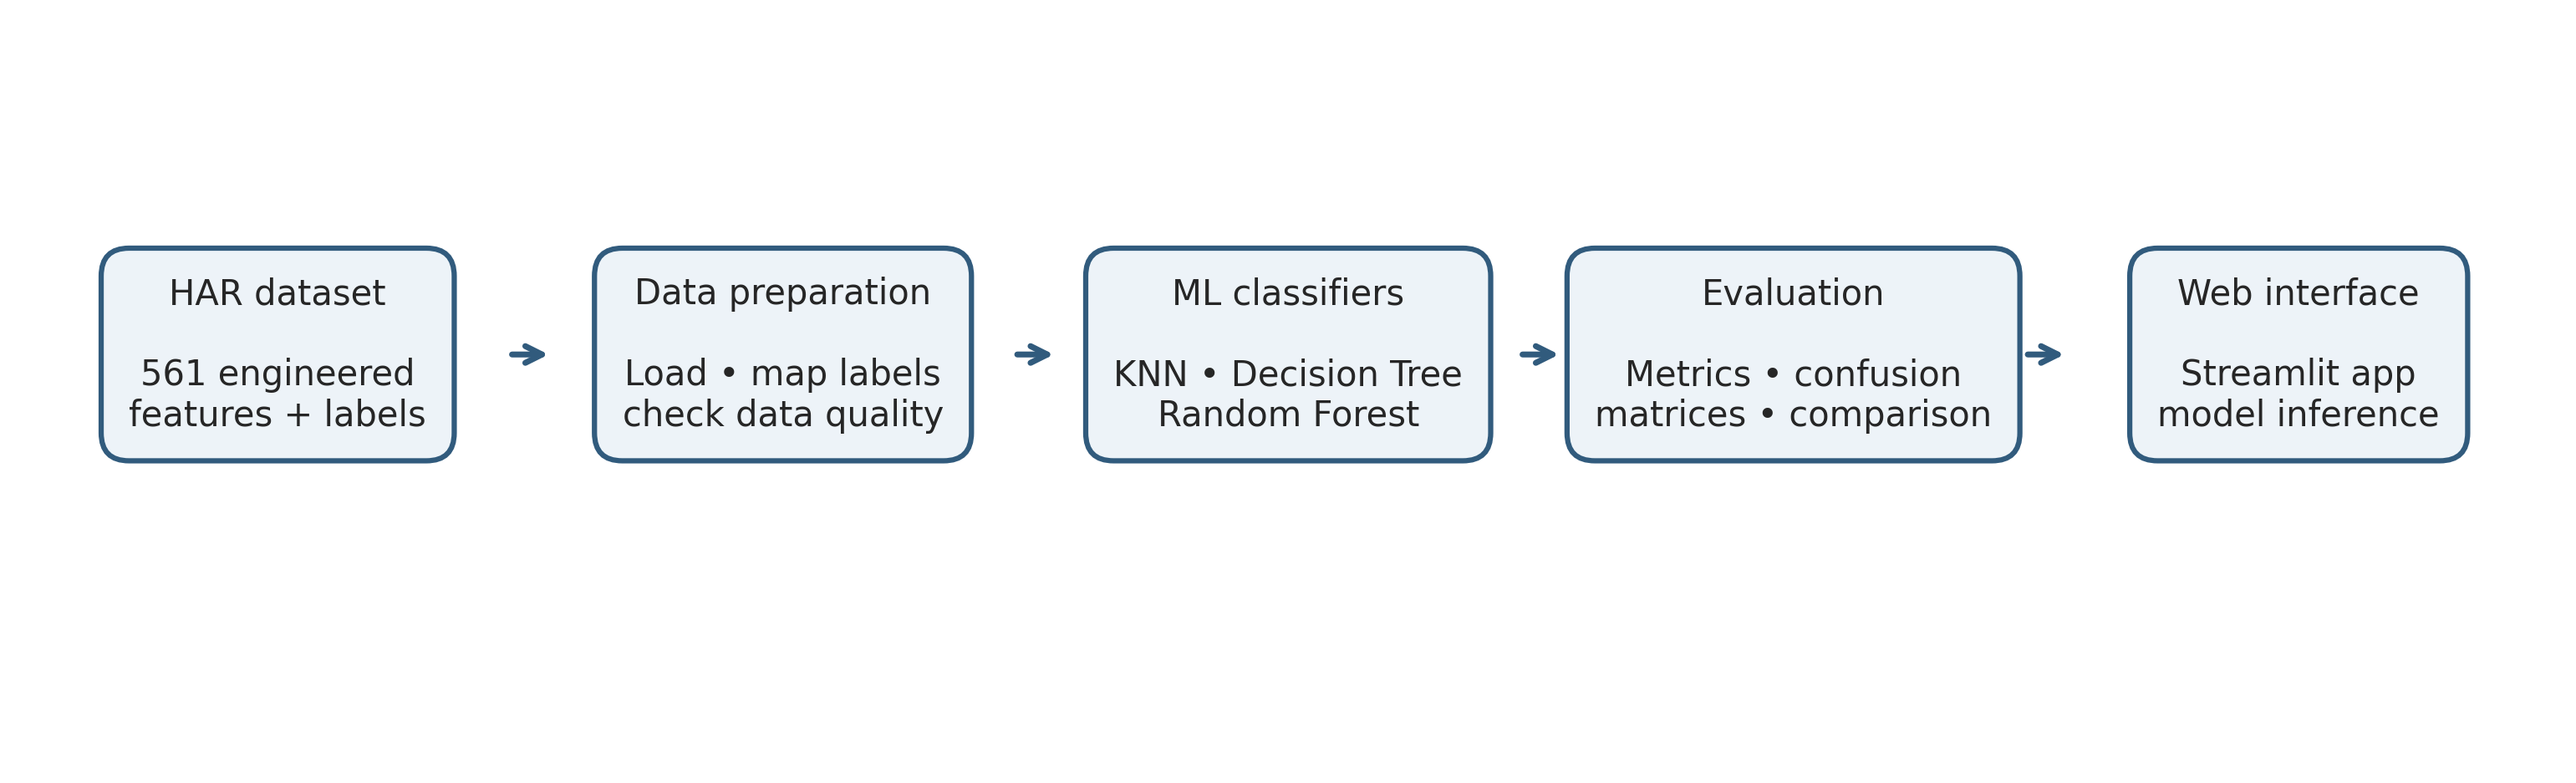
\includegraphics[width=\textwidth]{system_architecture.png}
\caption{High-level architecture of the HAR machine-learning workflow.}
\label{fig:architecture}
\end{figure}

\section{Software and Libraries}
The notebook uses Python and the following libraries: NumPy and Pandas for numerical and tabular data handling; Matplotlib and Seaborn for plots; Scikit-learn for preprocessing, model training and evaluation; and Joblib for saving trained models. The web application is hosted using Streamlit, according to the project URL supplied by the student.
